\chapter{?}
I det følgende afsnit vil lokalplanen for området ved Strøybergs Palæ beskrives, da denne sammen med kommuneplanen indeholder en række informationer om Strøybergs Palæ, og fastsætter rammerne for den kommende tilbygning. 
\newline \indent{     }   Til sidst vil der foretages en sammenligning mellem den førhen gældende lokalplan for området og den nuværende lokalplan, for at undersøge, hvilke ændringer der har været nødvendige at foretage, for at kunne realisere tilbygningen til Strøybergs Palæ.


\section{Lokalplan}
En lokalplan tager udgangspunkt fra en fremsat kommuneplan, og har til formål at styre udviklingen i et område. Lokalplanen skal give borgerne og byrådet et indblik i et bestemt område og give dem mulighed for at komme med tiltag til den fremlagte plan. Her fastsætter byrådet rammerne for, hvordan arealer, bygninger, beplantning, veje, stier m.fl. skal anlægges i et givent område. Lokalplaner skal ifølge planloven udformes af byrådet, der har pligt til dette, før der kan gennemføres større bygge- og anlægsprojekter.
\newline
\newline
En lokalplan indeholder punkterne; redegørelse, planbestemmelser og bilag.
\newline \indent{     }  Planen starter med en redegørelse, hvor lokalplanens baggrund og formål fastsættes og hele indholdet fremlægges. Der bliver også redegjort for miljømæssige forhold, hvordan lokalplanen forholder sig til andet byggeri, og om der kræves tilladelser eller anden slags dispensationer fra forskellige myndigheder.  
\newline \indent{     }   I lokalplanen informeres der om planbestemmelser, som er områdets fremtidige anvendelse. Dette illustreres via tekst og billeder.
\newline \indent{     }  Til sidst i lokalplanen ligger alle bilagene. Disse består oftest af forskellige kort (matrikelkort, arealanvendelseskort m.m.) samt forskellige tabeller omkring støj fra erhverv og trafik m.m. Bilagene er med til at uddybe og illustrere lokalplanbestemmelserne.
\newline
\newline
Byrådet kan til enhver tid udarbejde et lokalplanforslag. Når et forslag til lokalplanen er udformet, skal det offentliggøres i mindst otte uger, hvor borgerne kan komme med indsigelser eller forslag til ændringer. Efter de otte ugers offentliggørelse bedømmer byrådet, hvorvidt eventuelle indsigelser eller ændringer vil blive taget op. Dernæst vedtages planen, hvor den bekendtgøres i avisen og er hermed bindende for ejendommene, som ligger i lokalplanområdet.
\newline \indent{     }  Der må ikke laves ændringer i området i strid med lokalplanen, dog må eksisterende bebyggelser og anvendelse, der er etableret før lokalplanforslagets offentliggørelse, fortsætte. Endvidere er der ikke pligt til at gennemføre tiltag, der beskriver lokalplanen (\citep{lokalplan}, s. 4).

\section{Lokalplan 1-1-107}
Lokalplan 1-1-107 er lokalplanen for området ved Strøybergs Palæ. Lokalplanen er vedtaget af Aalborg Byråd den 12. november 2012, og offentligt bekendtgjort den 21. november 2012 (\citep{lokalplan}, s. 20).
\newline \indent{     }  Området for lokalplanen er ca. 1.200 $m^2$, og ligger ca. 100 m fra Limfjorden. Øst for lokalplanområdet ligger Gammel Havn, mod nord og vest ligger Utzon Parken og mod syd Nyhavnsgade. Ud over Strøybergs Palæ, der ligger i planområdet, er der også enkelte mindre bygninger, garager m.m. For at lokalplanen kan blive realiseret, skal mindre bygninger nedrives, hvis de ikke er bevaringsværdige (\citep{lokalplan}, s. 6). Området, som lokalplanen dækker, ses på Figur \ref{fig:1-1-107}.
\newline \indent{     }  Lokalplanen er udarbejdet med et ønske om, at lave en tilbygning til Strøybergs Palæ, hvor anvendelsesmulighederne i området således vil blive ændret til beboelse, serviceerhverv og kontorerhverv. Lokalplanen er udformet således, at den tager hensyn til, at den nye bebyggelse udformes efter den eksisterende bevaringsværdige bygning, eventuelt med et nutidigt arkitektonisk udtryk, således der er harmoni mellem den nuværende bygning og tilbygningen. Her tages der hensyn til bygningsskala, facaderytme og farve, da Strøybergs Palæ er vurderet til at være en bevaringsværdig bygning med en bevaringsværdi 4, som er middelværdi (\citep{lokalplan}, s. 5 og 9). Bevaringsværdien bestemmes på baggrund af fem værdier; arkitektonisk værdi, kulturhistorisk værdi, miljømæssig værdi, originalitet og tilstand, hvor vurderingen er givet i forhold til helhedsindtrykket af bygningens kvalitet og tilstand, dog vil den arkitektoniske- og den kulturhistoriske værdi veje tungest for bevaringsværdien. Bygninger med bevaringsværdi 2-4 er bygninger, som er fremtrædende grundet deres arkitektur, kulturhistorie og håndværksmæssige udførelse \citep{bevaringsvaerdi}. Lokalplanen fortæller desuden, at tage skal udføres som saddeltage eller som flade tage (\citep{lokalplan}, s. 17).
\newline \indent{     }  Lokalplanen indeholder to delområder, hvor delområdet A er hovedbygningen af Strøybergs Palæ, mens delområde B er sidebygningen dertil og et byggefelt liggende mod nord, hvilket er illustreret på Figur \ref{fig:aogb}. Inden for delområde A må ny bebyggelse opføres i 4 etager, samt en tagetage, og med en kælder maksimalt 1,25 m over terræn, som kan anvendes til parkering, depot og lignende. Inden for delområde B må ny bebyggelse opføres i 3 etager samt en tagetage og med en kælder maksimalt 2 m over terræn. I alt må tilbygningen højst være 19 m høj (\citep{lokalplan}, s. 7 og s. 16).

\begin{figure}[htbp]
	\centering
	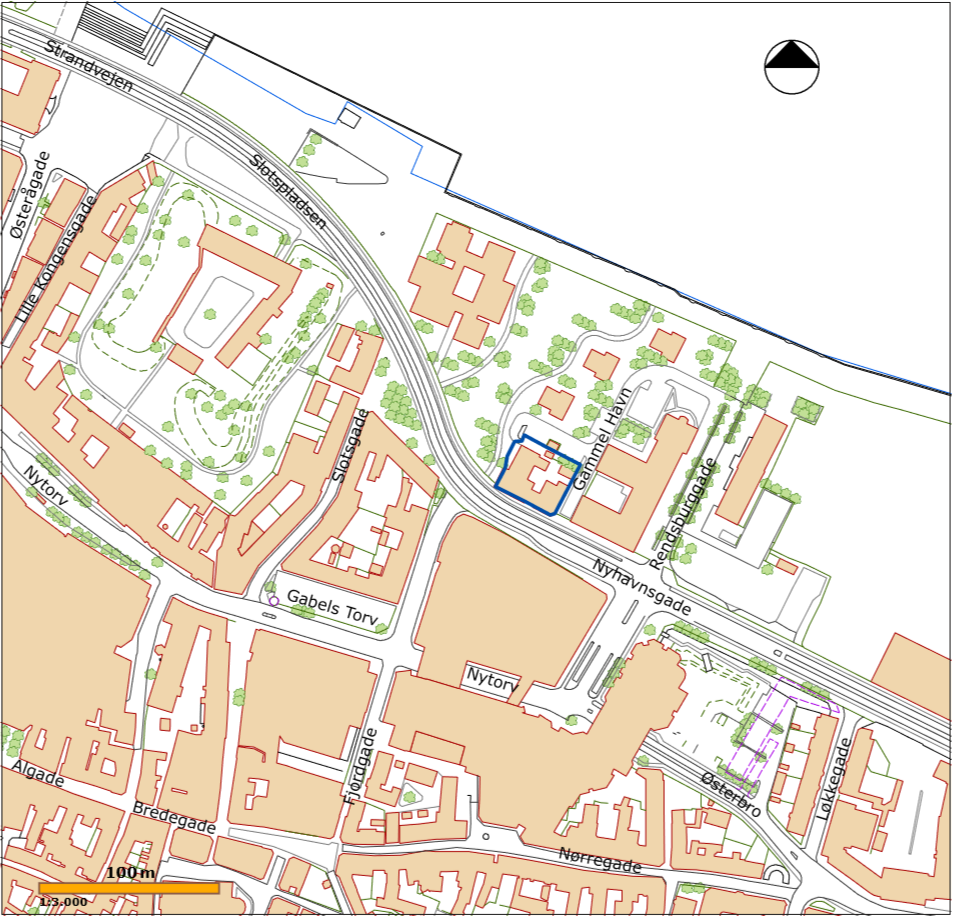
\includegraphics[width=0.5\textwidth]{billeder/nylokalplanoversigt.png}
	\caption{Lokalplan 1-1-107, lokalplanområde}
	\label{fig:1-1-107}
\end{figure}

\begin{figure}[htbp]
	\centering
	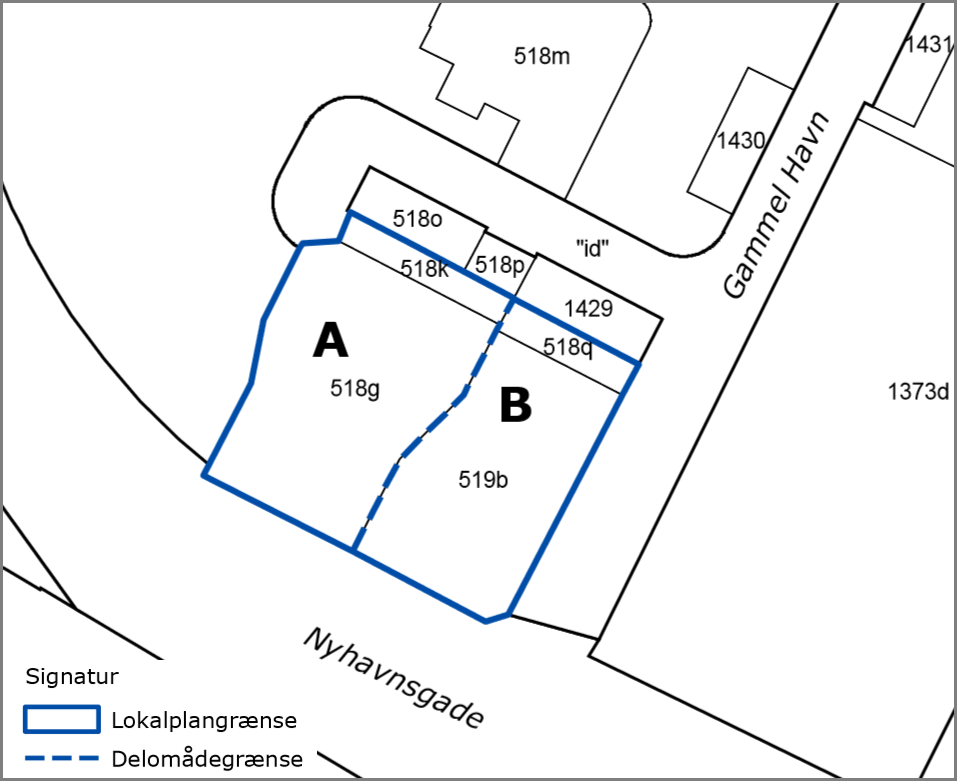
\includegraphics[width=0.5\textwidth]{billeder/tilbygning.png}
	\caption{Lokalplan 1-1-107, delområde A og B}
	\label{fig:aogb}
\end{figure}

Da lokalplanområdet ligger meget kystnært skal der i større grad dimensioneres efter klimatiske faktorer og ændringer. Her er hovedpunktet vandstandsstigning. Her tages der udgangspunkt i Aalborg Kommunes klimastrategi. Den forudsiger, at den generelle indre vandstand i nordjyske farvande vil kunne stige med op til 1 m. Derfor er der fastsat en minimum sokkelkote for stueplan på nye bygninger på 2,36 m DVR 90 grundet risikoen for vandstandsstigning (\citep{lokalplan}, s. 9).
\newline \indent{     }  Bygningen ligger placeret tæt op ad detailhandel og erhverv. Området benyttes af kollektiv trafik. Da bygningen ligger placeret ved Nyhavnsgade, kan dette give støjgener fra trafikken. Derfor skal der tages højde for dette, når der bygges. Det indendørs støjniveau må ikke overstige $L_{den}$ 33 dB, og ved udendørs opholdsarealer må den ikke overstige $L_{den}$ 58 dB. Støjisolering skal primært ske indvendigt, så bygningen ikke ændrer udseende. Overholdelse af de forskellige grænseværdier for støj skal kunne dokumenteres, før bygningen må tages i brug (\citep{lokalplan}, s. 8). Området er kortlagt på vidensniveau 1 og 2 efter jordforureningsloven. Et areal bliver kortlagt på vidensniveau 1, hvis der er kendskab til aktiviteter, der kan forårsage forurening på arealet. Det vil blive kortlagt på vidensniveau 2, hvis der er dokumentation for forurening i jord og grundvand på arealet \citep{vidensniveau}. Hvis der i forbindelse med bygge- og anlægsarbejde konstateres tegn på jordforurening, skal arbejdet standses og kommunens Teknik- og Miljøforvaltning skal underrettes. Herefter vurderes det, om der skal fastsættes vilkår, inden arbejdet kan genoptages (\citep{lokalplan}, s. 10).
\newline
\newline
Lokalplanen skal udarbejdes i samspil med den nuværende kommuneplan og anden fysisk planlægning i området omkring. Planen er, at der i lokalplanens område kan indrettes et mindre antal boliger. Det forventes at Aalborg Midtby får etableret 2.116 nye boliger i perioden 2008-2019. I bygningen kan desuden etableres butikker på maksimalt 250 $m^2$  og 500 $m^2$ pr. etage jf. kommuneplanen (\citep{lokalplan}, s. 8).

\subsection{Fra gammel til ny lokalplan}
I kraft med vedtagelsen af lokalplan 1-1-107 ophæves lokalplanen 10-082 for det område, som lokalplan 1-1-107 omfatter. På trods af, at de to lokalplaner omfatter to forskellige områdestørrelser, så er lokalplanerne fortsat ens på flere punkter, heriblandt miljøforholdene for området. Der er dog nogle små forskelle, og disse forskelle vil blive analyseret i det følgende afsnit. Nedenfor på Figur \ref{fig:10-082} ses lokalplanområdet for lokalplan 10-082.

\begin{figure}[htbp]
	\centering
	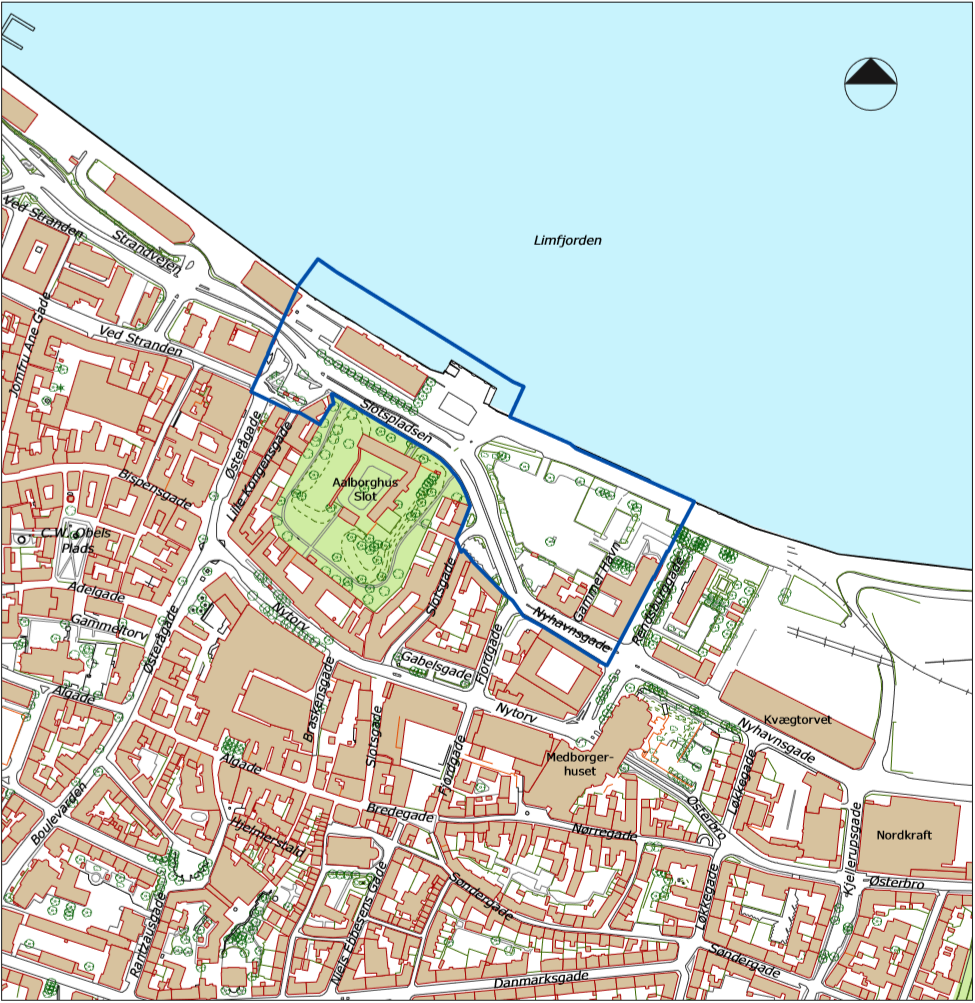
\includegraphics[width=0.5\textwidth]{billeder/lokalplanoversigt.png}
	\caption{Tidligere gældende lokalplan, 10-082, for området}
	\label{fig:10-082}
\end{figure}

I lokalplan 10-082 kan ny bebyggelse for området Strøybergs Palæ bygges i 4 etager samt tagetage med en maksimal højde på 22 m (\citep{gammellokalplan}, s. 19), hvor der i lokalplan 1-1-107 kan bygges i op til 3 etager samt tagetage for ny bebyggelse med en maksimal højde på 19 m. Denne ændring i højden kan skyldes, at der har været indsigelser imod de 22 m, da dette muligvis ville fjerne en udsigt eller sollys for de berørte personer. 
\newline \indent{     }  Der er i lokalplan 1-1-107 ligeledes taget højde for vandstandsstigning i Limfjorden, hvilket ikke er gjort i lokalplan 10-082. Grunden til dette kan skyldes, at der ikke tages højde for detaljerne, da lokalplan 10-082 foruden Strøybergs Palæ indeholder tiltag til Utzon Centeret, Slotspladsen og First Slotshotel.
\newline \indent{     }  Ligeledes bliver der præciseret i lokalplan 1-1-107, at isolering for trafikstøj ikke må ændre på facadens udseende, hvor der i lokalplan 10-082 blot står, at enhver ændring på bygningens facade kræver en tilladelse (\citep{gammellokalplan}, s. 19). En grund til at der først i lokalplan 1-1-107 står beskrevet, hvordan isoleringen skal foretages samt at facadeændringer kræver en tilladelse, kan være, at lokalplan 10-082 dækker over et større område end 1-1-107, og at detaljerne på tilbygningen dermed først er relevant for lokalplan 1-1-107. 
\newline \indent{     }  For ny bebyggelse og nye tilbygninger, som er omfattet af lokalplan 1-1-107, gælder det, at nye bygninger skal opføres i overensstemmelse med den eksisterende bebyggelse, dog gerne med nutidig arkitektonisk formsprog. Tilbygninger skal opføres i tilknytning til den eksisterende bevaringsværdige bygning, og skal derfor have det samme arkitektoniske udtryk, som bygningen i forvejen har. 
\newline \indent{     }  Dette punkt i lokalplanen forklarer de overordnede rammer for ny bebyggelse og tilbygning, men udover dette, er det mere frit for det pågældende rådgivningsfirma, at designe og konstruere de pågældende bygninger. De skal blot overholde lokalplanens givne rammer, hvorefter det kan diskuteres og fortolkes, hvor og hvornår grænsen for det arkitektoniske udtryk overskrides. Denne balance er derfor mest op til det rådgivende ingeniørselskab at fortolke.

\section{Delkonklusion}
Der er i de foregående afsnit redegjort for Aalborgs historie og baggrunden for byens udvikling. Ligeledes er der beskrevet, hvad en kommuneplan og lokalplan er, og der er lavet en dybdegående analyse af Aalborgs kommuneplan, med særligt fokus på Vækstaksen. Inden for vækstaksen ligger Strøybergs Palæ, som hører under den nuværende lokalplan 1-1-107, hvilken også er behandlet, analyseret og sammenlignet med den tidligere lokalplan for området, 10-0-82. Endelig er der foretaget en diskussion, hvor spørgsmålet stilles, hvorfor det er godt at udvikle i netop dette område, og derunder hvilken sammenhæng der er mellem Strøybergs Palæ og Vækstaksen.
\newline
\newline
Aalborg Kommune er vokset som by gennem tiden, og gennem den nuværende kommuneplan har kommunen en målsætning om, at blive Nordjyllands Vækstdynamo og blive en by med fokus på udvikling af studerende, erhverv, kultur med mere. 
\newline \indent{     }  Kommuneplanen er den overordnede ramme for byens udvikling, og den indeholder en 12-årig plan, hvor blandt andet målsætninger og planer er beskrevet. Kommuneplanen er opdelt i flere forskellige fokuspunkter, og den dækker derfor alt fra bæredygtighed og miljø til mobilitet og udvikling af samfundet. 
\newline \indent{     }  Under kommuneplanen findes lokalplanen, som beskriver et mindre område inden for kommunen og har til formål at styre udviklingen af dette. Lokalplanen skal stemme overens med kommuneplanens rammer, og der kan derfor ikke være modsigelser mellem de to planer. Opstår der komplikationer med udarbejdelsen af en lokalplan inden for en kommuneplans rammer, så anvendes der et kommuneplantillæg, for at løse problemet. De to planer er derfor tæt knyttet til hinanden, hvor kommuneplanen er den ledende af de to, men hvor der er sammenhæng mellem alle punkter i begge planer.
\newline
\newline
Vækstaksen beskriver et område i Aalborg, hvor der er planer om fremtidig udvikling. Disse områder består allerede i dag af virksomheder, uddannelsesinstitutioner, kulturattraktioner og andre interessepunkter for Aalborg Kommune. For Aalborg Kommune er det netop disse områder, som skal skabe den fremtidige vækst for Aalborg, og derfor er det fordelagtigt at udvikle yderligere i områderne. 
\newline \indent{     }  Med en beliggenhed inden for Vækstaksen, og i et af de planlagte vækstområder (se Figur \ref{fig:udvikling}), danner Strøybergs Palæ grundlag for en udvidelse. Ved at lave en tilbygning vil der blive plads til ekstra erhvervslokaler og lejligheder, og tilbygningen vil derfor være en medvirkende faktor til at styrke Aalborgs vækst.